\documentclass[]{aiaa-tc}% insert '[draft]' option to show overfull boxes

\usepackage{graphicx}
\usepackage{amsmath}

\usepackage{multicol}
\usepackage{blindtext}

\usepackage{subfig}
\usepackage{caption}
\captionsetup[subfigure]{labelformat=empty}

 \title{Large-Eddy Simulation of an over-expanded planar nozzle}

 \author{
 	Britton J. Olson
    \thanks{Graduate Student, Department of Aeronautics and Astronautics, Ph. (925) 550-3255} \  and 
  \ Sanjiva K. Lele 
  \thanks{Professor, Department of Aeronautics and Astronautics and Department of Mechanical Engineering, Ph. (650) 723-7721}\\
  {\normalsize\itshape
   Stanford University, Stanford, CA 94305}
 }

 % Data used by 'handcarry' option if invoked
 \AIAApapernumber{2011}
 \AIAAconference{41st AIAA Fluid Dynamics Conference and Exhibit, June 2011, Honolulu, Hawaii}
 % Shock-wave/boundary-layer interactions
 \AIAAcopyright{\AIAAcopyrightD{2011}}
 
 \lhead{ \scriptsize{41st AIAA Fluid Dynamics Conference and Exhibit \\ June 2011, Honolulu, Hawaii}}
 \rhead{ \scriptsize{Shock-wave/boundary-layer interactions}}
 
 
 % Define commands to assure consistent treatment throughout document
 \newcommand{\eqnref}[1]{(\ref{#1})}
 \newcommand{\class}[1]{\texttt{#1}}
 \newcommand{\package}[1]{\texttt{#1}}
 \newcommand{\file}[1]{\texttt{#1}}
 \newcommand{\BibTeX}{\textsc{Bib}\TeX}
 
 \newcommand{\divg}{\nabla\cdot}
\newcommand{\grad}{\nabla}
\newcommand{\V}{\vec{\mathbf{v}}}
\newcommand{\pd}[2]{\frac{\partial#1}{\partial#2}}
\newcommand{\pth}[1]{\left( #1 \right)}
\def\bgk#1{\mbox{\boldmath $#1$}}
\def\vec#1{\bgk{ #1}}
\def\ten#1{\underline{\bgk{ #1}}}

\begin{document}

\maketitle

\begin{abstract}

%\emph{
%We do a series of LES of Papam exp.  We show good agreement to exp. quantities and observe int. flow phenomenon not mentioned in exp.  We look at data and unsteady shock at level of detail that exp and RANS cant.}


Large-eddy simulation (LES) of an over-expanded planar nozzle is performed to elucidate the complex interaction between the turbulent boundary layer, the internal shock wave and the separated shear layer downstream of the shock.  A high-order compact differencing scheme, which includes artificial diffusivities for capturing discontinuities, is used to resolve turbulent structures while introducing very limited amounts of numerical dissipation.   This numerical simulation seeks to model one the experiments of Papamoschou et.al. and shed light on the underlying physics of the shock-boundary layer interaction and the Free-Shock Separation (FSS) which is present in over-expanded supersonic nozzles.  To achieve a feasible cost for computing a solution, the Reynolds number of the simulation is approximately $1/4^{th}$ of the experimental value and the geometrical ratio of the boundary layer thickness to throat is increased by a factor of two.  Simulation results compare well with those obtained from the experiment despite the modeling approximations.  The LES captures the unsteady fluctuation of the shockwave as it interacts with the incoming turbulent boundary layer and the separated shear layer downstream.  The richness of the simulation data allow for a more in-depth exploration of the underlying physics and have led to a better understanding of the unsteady shock wave behavior. 
\end{abstract}


%\begin{multicols}{2}


\section*{Nomenclature}

\begin{tabbing}
  XXXXXXXX \= \kill% this line sets tab stop
  $\beta$ \> bulk viscosity \\
  $C_f$ \> friction coefficient \\
  $\Delta\vec{x}$ \> grid spacing \\
  $\delta$  \> boundary layer thickness (99\% velocity thickness) \\
  $\ten{\delta}$ \> unit tensor \\
  $E$ \> total energy \\
  $\gamma$ \> ratio of specific heats \\
  $\vec{g}$ \> gravitational acceleration \\
  $\kappa$ \> thermal conductivity \\
  $H_t$ \> nozzle throat height \\
  $L_z$ \> domain extend in the span-wise direction \\
  $\mu$ \> dynamic viscosity \\
  $M$ \> Mach number \\
  $N_\xi,N_\eta,N_\zeta$ \> number of grid points in computational mesh \\
  $NPR$ \> nozzle pressure ratio, $p_{0_{i}}/p_\infty$ \\
  $p$ \> static pressure \\
  $\rho$ \> density \\
  $\vec{q}$ \> heat flux \\
  $R$ \> gas constant \\
  $Re$ \> Reynolds number \\
  $\ten{S}$ \> strain rate tensor \\
  $\ten{\tau}$ \> viscous stress tensor \\
  $t$ \> time \\
  $T$ \> static temperature \\
  $\vec{u}$ \> velocity vector \\
  $U_p$ \> Ideally expanded super-sonic velocity scale \\ 
  $\xi,\eta,\zeta$ \> generalized coordinate directions \\
  \\
  \textit{Subscript}\\
  $0$ \> total or stagnation value \\
  $e$ \> value at nozzle exit \\
  $\infty$ \> ambient or outer-nozzle conditions \\
  $i$ \> nozzle inflow conditions \\
  $N$ \> experimental nozzle value \\
  $+$ \> wall unit quantity \\
  $rr$ \> recycling-rescaling region \\
  $t$ \> value at nozzle throat \\
  $w$ \> wall value \\
 \end{tabbing}
 
 
% \end{multicols}
 
% \begin{multicols}{2}

%\vspace{4in}
\section{Introduction}

%\emph{ Shock waves affect the design of nozzle.... interaction with BL is not fully understood.  Exp. Papam sought to look at this phenomenon and found bla... RANS was used on this and found BLA... LES is very handy for this stuff.  We do LES.}

Internal shock waves are a major consideration in the design of supersonic devices.  In supersonic converging-diverging nozzles, the unsteady shock wave can become asymmetric and generate large ``side loads''~\cite{Ostlund:05} on the nozzle interior during engine start-up or under certain over-expanded conditions.  Although the occurrence of this phenomenon can be approximated, there is still a great deal which is not understood due to inherit complexities of the shock-boundary layer interaction.  Furthermore, the presence of shock waves inside a nozzle has recently been shown in experiments \cite{Papam:10} to enhance the downstream mixing of the nozzle jet.  Such an outcome might be desirable for engineering applications involving combustion related flows. 


The boundary layer separation caused by shock waves in the nozzle takes two forms.  The first, restricted shock separation (RSS), is typical of nozzles which contain a small internal shock (such as in thrust optimized nozzles) and which are over-expanded.  In this interaction, the flow separates from the wall and then reattaches forming a separation bubble.  This process is analogous to several other canonical shock boundary layer interactions~\cite{Dussauge:09,Bookey:05}.  The second, free shock separation (FSS), is common in ideally contoured nozzles and is unique in that the separated boundary layer fails to reattach downstream.  Rather there is a separated shear layer which persists down the length of the nozzle.  The coupling between the downstream separation region and the shock location is more complex for FSS than RSS and as a result is less understood\cite{Ostlund:05}.  Furthermore, the ``side loads'' tend to be largest in the FSS regime.

Recent experiments by Papamoschou et. al.\cite{Papam:09,Papam:10,Papam:06} of a planar nozzle have further elucidated the unsteady nature of the FSS.  Interesting flow features such as an asymmetric lambda-shock structure in the nozzle and largely enhanced mixing in the downstream jet of over-expanded nozzles have been observed.  These experiments found a broad-band range of frequencies present in the shock's motion.  The higher frequencies are independent of the shock strength/location and are governed by the incoming turbulent boundary layer.  The lower frequencies, however, depend greatly on the shock strength and the shock location oscillates with a larger amplitude with increasing shock strength.  The experimental data show a very intuitive correlation between the shock location and total pressure fluctuation downstream of the shock.  As the shock moves up/down stream, the strength of the shock will vary, thus altering the total pressure loss in the flow.  However, the available time resolved measurements of the turbulent boundary layer and the separated shear layer downstream are limited.  Thus, the effect of the boundary layer on the shock motion, and subsequently the separated shear layer, cannot be quantified.  Although, this effect could be small, recent studies of similar flows have shown that turbulent structures do indeed effect the low frequency shock motion~\cite{Touber:09}.  To our knowledge, the only simulation of this experiment was performed by Xiao et al \cite{Xiao:07}, which constituted a steady two dimensional Reynolds Averaged Navier-Stokes (RANS) solution.  That study had agreeable results with the mean statistics of the experimental data.  However, as is the nature of steady RANS, unsteady phenomenon were not captured and no additional insights about the unsteady coupling between boundary layer, shock location and downstream shear layer were made.

Large Eddy Simulation (LES) has recently had excellent success in capturing the unsteady flow physics of shock wave boundary layer interactions.\cite{Morgan:10b,Kawai:10aiaa,Touber:09,Pirozzoli:09}  Favorable comparison to experiments at ever increasing Reynolds numbers is demonstrating that LES is a valuable tool for engineering design analysis and fundamental scientific research.  We have leveraged this technique to generate a rich data set which can be interrogated at a higher level of sophistication than is possible with experimental data or RANS.  We provide a brief summary of the methodology for the LES we are conducting and present results of a grid refinement study for capturing the incoming turbulent boundary layer.  Results from LES show excellent agreement with the experimental data.  We also report observations made from the numerical Schlieren and offer an intuitive hypothesis for the mechanism governing the low frequency shock motion.  


%\end{multicols}
%\clearpage
%\begin{multicols}{2}


\section{LES Methodology}

\subsection{Governing Equations}

The compressible Navier-Stokes  equations can be written as

\begin{equation}
  \pd{\rho}{t} + \divg \pth{ \rho\bgk{u} }  = 0 ,
  \label{eq:mass}
\end{equation}
\begin{equation}
  \pd{\rho\bgk{u}}{t} + \divg \pth{ \rho\bgk{u}\bgk{u} + \ten{\delta} P - \ten{\tau} } = \rho\bgk{g} ,
  \label{eq:mom}
\end{equation}
\begin{equation}
  \pd{E}{t} + \divg \pth{ \bgk{u}\pth{E+p} - \bgk{u}\cdot\ten{\tau} + \vec{q}  }  = \rho\bgk{u}\cdot\bgk{g}
  \label{eq:energy}
\end{equation}


where


\begin{align}
	\ten{\tau} &= 2 \mu \ten{S} +(\beta-\frac{2}{3}\mu) \pth{\divg\bgk{u}}  \ten{\delta}, \\
	\ten{S} &= \frac{1}{2} \pth{  \grad \bgk{u} + \pth{ \grad \bgk{u}}^T }  ,\\
        \vec{q} &= - \kappa \grad T, \\
	E &=  \frac{p}{\gamma-1} + \frac{1}{2}\rho \bgk{u}\cdot\bgk{u}, \\
	T &= \frac{p}{\rho R}
\end{align}

Equations~\ref{eq:mass}-\ref{eq:energy} are numerically solved in conservation form on a generalized curvilinear grid.  Values are computed with dimensional units and air ($\gamma=1.4$) is used as the working fluid.

\subsection{Numerical Methods}


All first derivatives comprising the gradient and divergence operators in the governing equations are computed using a 10th-order compact central differencing scheme \cite{Lele:92}.  The high wave-number resolution of this scheme is desirable in the boundary and shear layers were turbulent fluctuations need to be resolved.  High-wave-number-biased artificial diffusivities \cite{Kawai:10,Cook:07,CookCabot:05} are used to smooth out sharp discontinuities (such as shock waves) in the flow and act as the sub-grid scale model.  In the future, we plan to more closely examine the effects of explicit sub-grid models.  These diffusivities are modified to alleviate the prohibitive numerical stiffness which arises in the high aspect-ratio grid near the viscous boundary layer and shock.

The equations are advanced in time using a 5-stage, fourth-order Runge-Kutta scheme\cite{Kennedy:00} chosen for its broad stability properties in both convective and diffusive terms.  At the completion of every sub-iteration, an 8th-order filter is applied to the conserved variables to remove the top $1/10^{th}$ of wave numbers as sharply as possible.  The Courant-Friedrichs-Lewy (CFL) stability limit is near unity for the entirety of the calculation.

\subsection{Mesh}

The computational mesh is generated by mapping a single structured mesh to the boundary on the planar nozzle.  The same mesh then diverges and coarsens to form a background mesh which models the far-field conditions of the experiment.  The corner radius where the background domain meets the nozzle is the size of the turbulent boundary layer, $\delta$, whereas the experimental corner was much sharper.  The converging portion of the nozzle is also modeled and is discussed in the following section.   
For the given resolution requirements in Table~\ref{tbl:mesh}, a nozzle height Reynolds number of $90\times 10^3$ is used.  This Reynolds number is approximately four times smaller than that observed in the experiment.  Table~\ref{tbl:mesh} shows parameters of mesh A, B and C which define the wall spacing in viscous units and give the overall grid size.  

\begin{figure}[!htb]% order of placement preference: here, top, bottom
	\centering
  	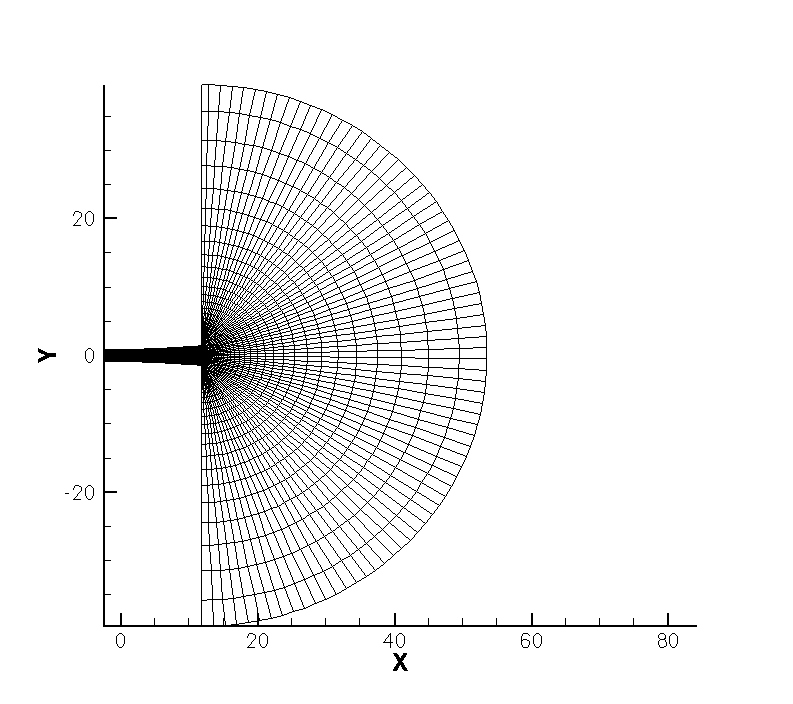
\includegraphics[width = 3in]{figs/full5.png}
	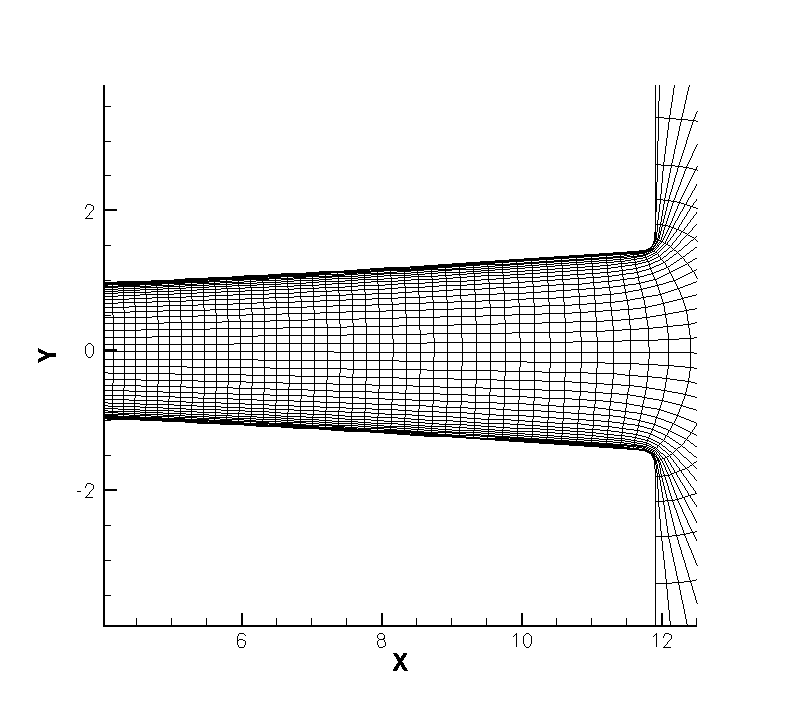
\includegraphics[width = 3in]{figs/zoom10.png}
	\caption{Computational mesh showing every 5th gridline in the over all domain (left) and every 10th grid line in the diverging section of the nozzle(right).  }
 	\label{fig:mesh}
\end{figure}

It was determined to be computationally infeasible to run a wall resolved LES at the actual Reynolds number of the experiment while keeping the boundary layer the same size.  The most prohibitive attribute of such a computation is the time integration.  Given the small viscous length scale required near the wall and the CFL condition imposed for numerical stability, the amount of time steps required to capture the low frequencies reaches the millions.  For the domain size required, this would be an extremely expensive computation in both duration and scale.  
Increasing the boundary layer thickness and reducing the Reynolds number is one solution we have chosen.  Another approach that is planned for future investigation is performing a wall modeled LES.  Doing so decouples the wall resolution from the viscous inner scales and reduces the computational cost substantially.

%For the viscous boundary layer to be be resolved near the wall, the length scale becomes order $\delta_{99}/Re_{\tau}$.  Furthermore, to capture the low frequency motion, the calculation must be run for several periods, in our case this is order $\approx 100 H_t/U_p$.  Assuming the time step is chosen such 


\subsection{Boundary Conditions}

The far field uses a non-reflecting characteristic boundary condition\cite{Poinsot:92}.  Furthermore a ``buffer'' region is applied at the last few grid points which smoothly damps the flow to ambient conditions without reflections.  The nozzle walls are viscous (no slip) and adiabatic, e.g. $\vec{u}_w=0$ and $\vec{q}_w\cdot\vec{n}_w = 0$.  The span-wise direction is periodic, which is an approximation to the experimental geometry which has side walls.  It is computationally infeasible (for the present LES) to resolve the boundary layer of the entire converging section of the nozzle.  Therefore, the computational domain begins at the throat of the nozzle and we use the method of recycling-rescaling\cite{Lund:98,Urban:01} to continuously feed the simulation an accurately evolving turbulent boundary layer.  The boundary layer thickness to nozzle throat height ratio ($\delta/H_t$) exceeds the observed experimental ratio by a factor of 2.  At the throat this gives a momentum thickness Reynolds number of 1100.  The mean inlet variables ($\vec{u}$, $p$,$\rho$) are given by the quasi-1d approximation.  Figure~\ref{fig:info_3d} shows the inflow and nozzle portion of the domain and depicts the recycling-rescaling section.


%\end{multicols}
\begin{table*}[!h]

\begin{center}
	\caption{Computational mesh parameters for various levels of refinement.  The value of $L_z$ of the experiment\cite{Papam:10} was $3.5H_t$.
	\label{tbl:mesh}
	}
	\begin{tabular}{lcccccccr}
	%\multicolumn{11}{c}{Mesh} \\ 
	\hline 
	Mesh & $N_{\xi}$ & $N_{\eta}$ & $N_{\zeta}$ & $L_z$ & $\Delta x^+_{in}$ & $\Delta y^+_{in}$ & $\Delta z^+_{in}$ & Total Pts.\\
	\hline 
	A & 512 & 128 &              128            & 1.5$H_t$ & 40 & 1-55 & 30 & 8.39 M \\
	B & 768 & 256 &              256           & 2.0$H_t$ & 30 & 1-23 & 20 & 50.33 M \\
	C & 1024 & 386 &              386            & 2.3$H_t$ & 20 & 1-14 & 15 & 152.6 M
	\end{tabular}
\end{center}
\end{table*}

%\begin{multicols}{2}


%\end{multicols}



%\clearpage

\begin{figure}[!htb]% order of placement preference: here, top, bottom
	\centering
  	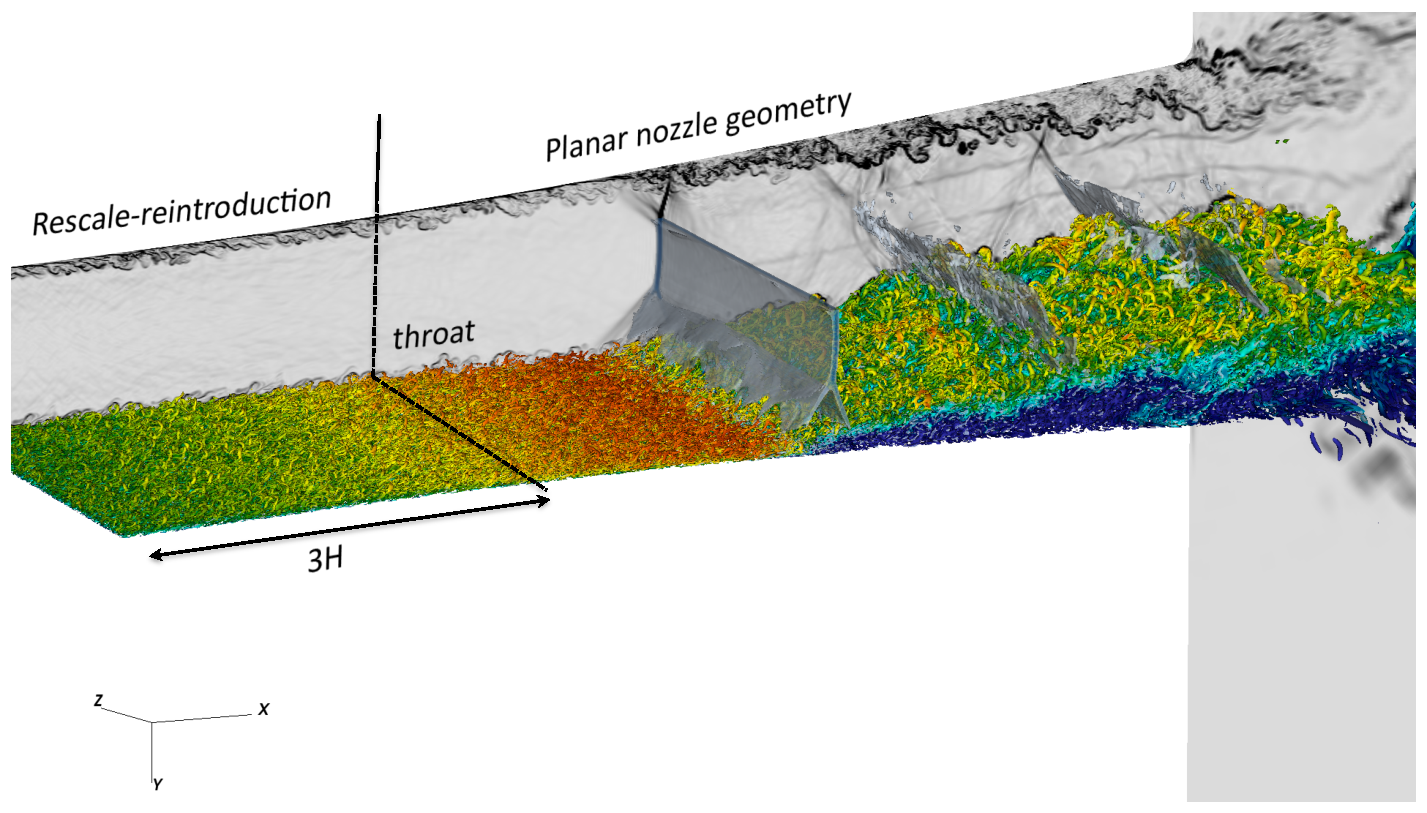
\includegraphics[trim = 0in 1.2in 0in 0in, clip, width = 7in]{figs/info_slide2.pdf}
	\caption{Iso-volume of the Q-criterion colored by Mach number show the incoming turbulent boundary layer and the large separated shear layer.  The shock is visualized by an iso-volume of $\nabla\cdot\vec{u}$.  The back plane shows a slice of $||\nabla\rho||$, depicting the smaller shear layer.  The throat location is indicated as is the region which recycles and rescales the incoming turbulent boundary layer.}
 	\label{fig:info_3d}
\end{figure}

%\begin{multicols}{2}

\clearpage
\section{Experimental Setup}


The particular experimental configuration modeled by the present LES was published the Johnson and Papamoshcou.~\cite{Papam:10}.  The geometry for the diverging section is fully defined by the given throat height, $H_t$ and area ratio, $A_e/A_t$.  The contour of the nozzle is simply the solution to a 4th order polynomial with boundary conditions.  Furthermore, the measure of the nozzle's over-expansion is given by the ratio of reservoir total pressure to ambient total pressure, or the nozzle pressure ratio (NPR=$p_{0,res}/p_{0,amb}$).  The present LES models case 3 from this experiment with an area ratio of 1.6 and NPR of 1.7.  This configuration had the most experimental data available and also generated large asymmetries in both the shock structure and the subsequent separated shear layer.  

Measurement devices included an array of static pressure ports on the nozzle wall.  A dynamic pitot tube was used to obtain a centerline mean pressure profile and total pressure rms values in the separated shear layer.  Four of the static pressure ports were simultaneously sampled at a frequency of 30 kHz.  This instantaneous pressure profile was fit to a characteristic shape resembling a shock-wave.  Doing so, yielded an approximate location for the shock wave and thus a time history of the shock location.  Johnson~\cite{Papam:10} showed that the shock position time history was insensitive to the particular shape used in the fit.  High resolution Schlieren images of the diverging section and the exit plume of the nozzle were also captured.

%\end{multicols}

\begin{figure}[!h]% order of placement preference: here, top, bottom
	\centering
  	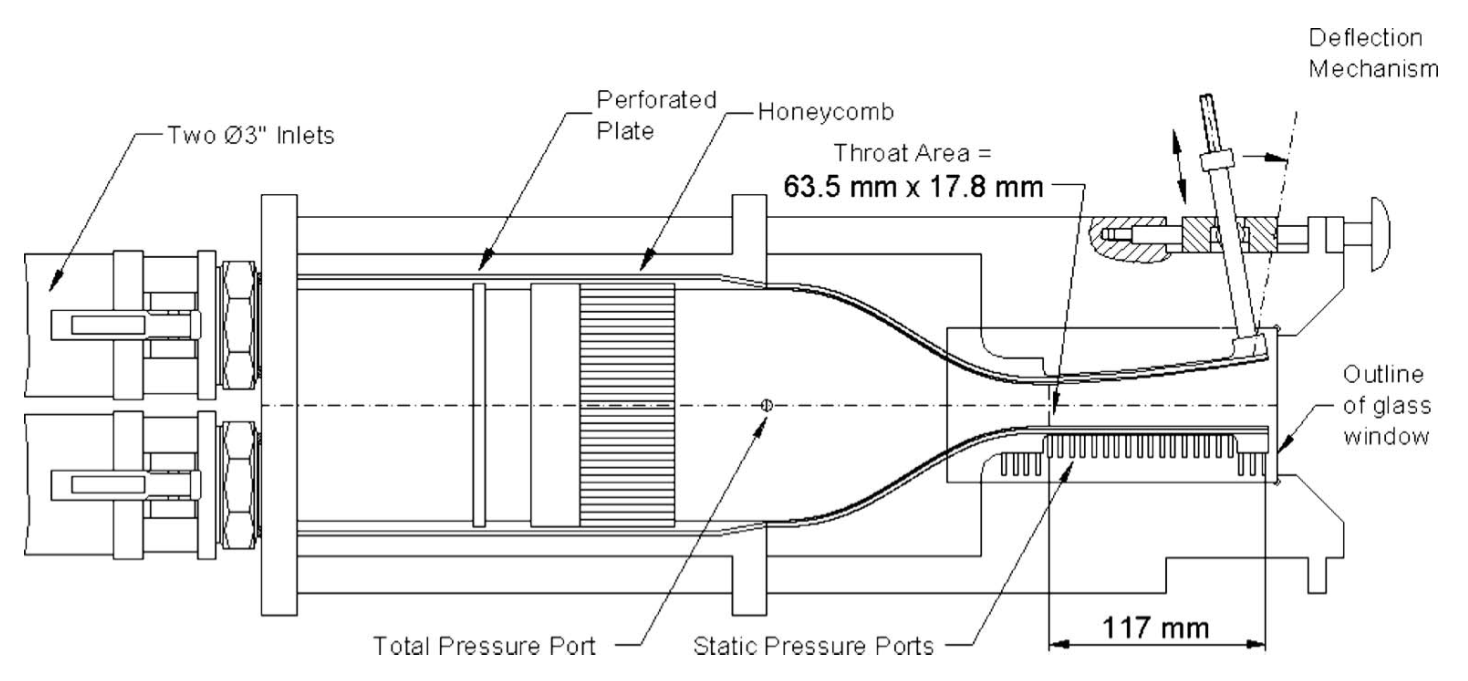
\includegraphics[width = 6in]{../../data/experiment/exp_setup.png}
	\caption{Experimental setup~\cite{Papam:10} showing the converging and diverging section of the nozzle.  The present LES only explicitly models the diverging section and uses recycled turbulence and the quasi-1D equations to model the converging portion. }
 	\label{fig:exp_setup}
\end{figure}

%\begin{multicols}{2}

\clearpage
\section{Results}

The accuracy of our LES calculation must be established before these data can be used to confidently explore the underlying physics.  This accuracy is measured by comparing against experimental data and performing a mesh refinement study.  Data from the mesh refinement study show the incoming turbulent boundary layer is being captured well.  The periodic span-wise direction, although not truly periodic in the experiment, is sufficiently large for flow structures to be independent of the periodic boundary.  Furthermore, our LES calculations show excellent agreement with both the mean and time dependent quantities from the experiment.  The aforementioned results are shown here to establish the fidelity of our LES database.

%Unless otherwise stated, results from mesh A are assumed for the reported data as this case has, thus far, the largest time history available.  Convergence studies of the long-time scale behavior are the topic of future research.

%Preliminary results from the coarse mesh simulation are presented here.  The computation ran on 256 processors for 2 days which was long enough to wash out initial transients, develop the boundary layer and capture the low frequency oscillations of the shock location.  The coarse calculation attempts to match the particular experimental configuration from Papamoschou et.al.\cite{Papam:09} with a given nozzle pressure ratio ($NPR$) of 1.77 and an area ratio ($A_e/A_t$) of 1.4.  Figure~\ref{fig:info_3d} shows the main features of the over-expanded nozzle experiment.  A normal shock wave is set up inside the nozzle and forces the turbulent boundary layer to separate.  The flow does not reattach and there is a large shear layer downstream as the flow exits into the ambient conditions outside the nozzle.

\subsection{Incoming Turbulent Boundary Layer}

The incoming turbulent boundary layer is well captured by the LES case A and B.  Viscous length scales near the wall are explicitly modeled with varying grid spacing by cases A, B and C.  These spacings are given in viscous wall units in Table~\ref{tbl:mesh} for the different resolution cases.  Mean velocity and RMS profiles (Fig.~\ref{fig:BL_prof}) for the B and C meshes are nearly identical.  The momentum thickness Reynolds number, $Re_\theta$ was 1100.  Case A is shifted upward, indicating a lack of resolution near the wall.  It is also important to note here, the shift upward from the standard log-law fit ($U_{VD}^+ = \log(y^+) / \kappa+ b $), where $\kappa$ is the Von Karman constant and $b$ is the intersect.  The converged profile of the calculations is shifted from the common parameters for $\kappa$ and $b$ of 0.41 and 5.2 respectively.  This is attributed to the substantially large pressure gradient present at the throat.  Spalart~\cite{Spalart:93} investigated the effect of a favorable pressure gradient on the velocity profiles in the boundary layer and found that for a normalized pressure gradient of $\frac{dP}{dx}\frac{\delta}{\tau_w} = -0.3$ there was an observed shift in $\kappa$ of 8\%, as $b$ is kept constant.  The pressure gradient at the throat for the current study was $\frac{dP}{dx}\frac{\delta}{\tau_w} = -0.7$ and the observed shift is 10\%.  Figure~\ref{fig:dPdx} shows a comparison in mean velocity profiles between the present LES and the DNS of Spalart.  Furthermore, this shift of $\kappa$ for both the present LES and DNS of Spalart are within the predicted range given recently by Dixit and Ramesh~\cite{Dixit:08}.  The results of Spalart and the converged LES profiles indicate that the calculation is accurately capturing the boundary layer and the effect of the favorable pressure gradient.  In the converging section of the throat, the LES does not model the geometry and hence will have a different pressure gradient than the experiment (Fig.~\ref{fig:dPdx}).

%\end{multicols}



%\begin{multicols}{2}

Downstream of the throat, the pressure gradient remains favorable.  This sustained acceleration of the flow causes the profiles to tend toward re-laminarization.  Neither experiment or the LES actually re-laminarize yet there is a clear shift in the mean profiles that could potentially effect the shock motion.  Figure~\ref{fig:stations} shows mean velocity profiles at various stations between the throat ($x/H_t=0$) and mean shock location ($x/H_t=3.5$).


\begin{figure}[!ht]
	\subfloat[(a)]{\includegraphics[height=2.5in]{../../figs/mean.pdf}}
	\subfloat[(b)]{\includegraphics[height=2.5in]{../../figs/rms.pdf} }
	\caption{ {\bf Left:} Mean velocity profile (Van Driest transformed) in the wall normal direction ($+$ units) for the cases of mesh A (dashed), B (dashed-dot) and C (solid) at the nozzle throat.  Inner and log-law fits are plotted for reference.  {\bf Right:} Diagonal components of the Reynolds stress for the three cases.
	\label{fig:BL_prof}
	}
\end{figure}


\begin{figure*}[!ht]
	\subfloat[(a)]{\includegraphics[height=2.5in]{../../figs/dPdx.pdf}}
	\subfloat[(b)]{\includegraphics[height=2.5in]{../../figs/spalart.pdf}}
	\caption{ {\bf Left:} Normalized wall pressure gradient ($\frac{dP}{dx} \frac{\delta^*}{\tau_w}$)from the experiment (circles) and the LES (dashed) showing agreement beyond the throat location ($x=0$) and its favorable nature.  {\bf Right:} Mean velocity profiles from the present LES (solid) and DNS performed by Spalart~\cite{Spalart:93} showing expected upward shift in the boundary layer profile.
 	\label{fig:dPdx}
	}
\end{figure*}



\begin{figure*}[!ht]
	\begin{centering}
	\includegraphics[height=3.75in]{../../figs/mean_st.pdf}

	\caption{ Mean velocity profiles (Van Driest) at various stations along the length of the nozzle.  The sustained favorable pressure gradient causes a further shift upward in the mean profiles.
 	\label{fig:stations}
	}
	\end{centering}
\end{figure*}


\clearpage
\subsection{Mean Pressure Profiles}
The LES mean pressure profiles at the centerline and at the wall compare well to the experimental data.  Upstream of the nozzle throat, centerline pressure does not agree with the experiment.  This is expected, as our approach models the converging section using the quasi-1d flow relations and the method of recycling-rescaling for the inflow variables and turbulent boundary layer.  Figure \ref{fig:P_prof} shows good agreement with the experimental data after the throat ($x=0$) indicating that the modeling of the converging section has a minimal effect on the flow past the throat.  The modeled converging section does however, shift the virtual throat location of the nozzle upstream by 2\% of the nozzle length.  This shift is accounted for in the remainder of the data and was constant for all three LES cases.  The oscillations behind the shock are resolved compression and expansion waves which are physical and which persist after long time averaging.

\begin{figure*}[!ht]
	\subfloat[ (a) ] {\includegraphics[height=2.5in]{../../figs/Pcenter.pdf} }
	\subfloat[ (b) ] {\includegraphics[height=2.5in]{../../figs/Pwall.pdf} }
	\caption{ Mean pressure profiles from the experiment (circles),  LES case A (dashed) and LES case B(dashed-dotted) along the centerline (left) and wall (right). 
	\label{fig:P_prof}
	}
\end{figure*}


\subsection{Span-wise extent and the turbulent shear layer }
As previously mentioned, the LES calculations use periodic boundary conditions in the span-wise($z$) direction.  This approximates the experiment which has physical walls on these boundaries.  The aspect ratio of the experiment (width to height at the throat) was $\approx 3.5$ and the effect of this quantity on the shock-wave behavior is unknown.  It is expected the span-wise domain must be sufficiently large in order to represent the large structures in the flow.  A smaller domain will directly impact the dynamics and evolution of the flow.  To determine the length scales present in the nozzle, a two-point correlation of stream-wise velocity, span-wise velocity and pressure was computed and averaged over time for 2 locations in the flow.  Figure~\ref{fig:span_corr} shows $R_{11}$ of pressure in the span-wise direction (normalized by span extent, $L_z$) at a location in the boundary layer ahead of the shock and in the separated shear layer.  The other variables are not shown here but exhibited similar behavior to the pressure correlation.  The correlations have substantially decayed for the regions in both the boundary layer and the shear layer, indicating sufficient span length, $L_z$.  

Figure~\ref{fig:span_spec} shows the spectra for these same two location and the three mesh resolutions.  The spectra indicate the range of energetic scales present in the shear layer is substantially larger than in the boundary layer.  The lack of collapse of the spectra for the three meshes is somewhat expected given the slight difference in probe location among the meshes and quantity of temporal data available for each mesh.  Mesh A has several low frequency periods of data while mesh B has only one.  Mesh C has yet to complete as entire low frequency oscillation.  The probe locations can been seen in Figure~\ref{fig:mean} and \ref{fig:RMS} which show mean and rms values for the flow variables for the various meshes.  Taking into account that the large shear layer between cases A and B is located on opposite sides, the results are qualitatively agreeing between the two meshes.  One clear distinction between the two averaged solutions is the diffuseness of the shock for case B.  This can be seen by comparing the static pressure of the two meshes in Figure~\ref{fig:mean}e-f.


%Furthermore, the Taylor microscale, $\lambda_g$ is a function of $R_{11}$ and is calculated on a sub-domain of the diverging section.  Contours of $\lambda_g$ are shown in Figure~\ref{fig:span_corr} for the coarse and medium resolution cases.  The incoming turbulent boundary layer, as expected, has the smallest length scales.  The location directly downstream of the normal shock and in the region directly between the shear layers has the largest values for $\lambda_g$.  For the coarse and medium resolutions the value of $\lambda_g / L_z$ doesn't exceed 0.2.  The decay of $R_{11}$ and small maximum values of $\lambda_g/L_z$ indicate that the effect of the span has a diminishing effect on the structures.

%\end{multicols}


\begin{figure}
	%\centering
	\hspace{-.65in}
	\subfloat[(a) Stream-wise velocity, mesh A]{ \includegraphics[width=3.75in]{../../figs/u_mean_cor.pdf}}
	\subfloat[(b) Stream-wise velocity, mesh B]{ \includegraphics[width=3.75in]{../../figs/u_mean_med.pdf}}
	
	\hspace{-.65in}
	\subfloat[(c) Vertical velocity, mesh A]{ \includegraphics[width=3.75in]{../../figs/v_mean_cor.pdf}}
	\subfloat[(d) Vertical velocity, mesh B]{ \includegraphics[width=3.75in]{../../figs/v_mean_med.pdf}}
	
	\hspace{-.65in}
	\subfloat[(e) Static Pressure, mesh A]{\includegraphics[width=3.75in]{../../figs/p_mean_cor.pdf}}
	\subfloat[(f) Static Pressure, mesh B]{ \includegraphics[width=3.75in]{../../figs/p_mean_med.pdf}}
	\caption{ Time averaged flow quantities showing the results from mesh A (left) and mesh B (right).  Mesh C contains far too few temporal data for reasonable temporal averaging.  The contour plots show probe locations in black for data shown in Figure~\ref{fig:span} and are normalized by the ideally expanded velocity scale ($U_p$) and ambient pressure.
 	}
	\label{fig:mean}
\end{figure}


\begin{figure*}[!ht]
	\centering
	\subfloat[(a)]{\label{fig:span_corr} \includegraphics[height=2.5in]{../../figs/corr_span_p.pdf}}
	\subfloat[(b)]{\label{fig:span_spec} \includegraphics[height=2.5in]{../../figs/spec_span_u.pdf}}
	\caption{ {\bf Left:} Two point auto-correlation for pressure fluctuation in $z$ vs. distance for a point in the pre-shock boundary layer (black) and large separated shear layer (blue), for mesh A (dashed), B (dashed-dot) and C (solid).  
	{\bf Right:} Energy spectra for the same two locations and 3 resolutions with identical color coding as in Fig.~\ref{fig:span_corr}.
 	}
	\label{fig:span}
\end{figure*}


%\begin{multicols}{2}

With sufficient domain size, the LES captures the energy containing scales of the separated shear layer well.  Total pressure fluctuations were recorded in the large separated shear layer ($x=x_{exit}$ and $y/H_t = 0.32)$ in the experiment.  Figure~\ref{fig:PSD_comp} shows the power spectral density (PSD) from the experiment and LES case at an identical probe location.  Agreement is good and shows that the energy containing scales and their cascade are being accurately captured.  


\begin{figure*}
	\centering
	\includegraphics[height=3.75in]{../../figs/PSD_compare.pdf}
	\caption{ Power Spectral Density (PSD) at a point in the large separated shear layer for the LES (solid) and experiment (circles) vs. Strouhal number.  The LES captures the PSD over a large frequency range extremely well, indicating the method is capturing the significant energy containing scales.
 	\label{fig:PSD_comp}
	}
\end{figure*}


\begin{figure}
	%\centering
	\hspace{-.65in}
	\subfloat[(a) Stream-wise velocity fluctuations]{ \includegraphics[width=3.75in]{../../figs/uu_cor.pdf}}
	\subfloat[(b) Vertical velocity fluctuations]{ \includegraphics[width=3.75in]{../../figs/vv_cor.pdf}}
	
	\hspace{-.65in}
	\subfloat[(c) Span-wise velocity fluctuations]{\includegraphics[width=3.75in]{../../figs/ww_cor.pdf}}
	\subfloat[(d) Reynolds shear stress]{ \includegraphics[width=3.75in]{../../figs/uv_cor.pdf}}
	
	\centering
	\subfloat[(e) Total Pressure fluctuations]{ \includegraphics[width=3.75in]{../../figs/ptpt_cor.pdf}}
	\caption{ Time averaged fluctuating quantities depict the asymmetry of the shear layer for mesh A.
 	}
	\label{fig:RMS}
\end{figure}

\clearpage
\subsection{Shock wave motion}

A primary feature of the planar nozzle flow field is the large internal shock wave.  Capturing the unsteady motion of the shock is necessary to fully quantify the underlying physical processes of the flow.  Here we show three comparisons to experimental data that demonstrate the shock is being adequately represented by the LES.  The three comparisons are: 1) wall pressure, 2) time history of the shock location and 3) Schlieren.



\subsubsection{Wall pressure}

To compare ``apples to apples'' with the experimental data, we extract wall pressure time histories from the data set, just as the experimentalist have done.  The compensated energy spectra, $kE(k)$, are computed for each probe location along the $x$-direction on the wall which has the larger separated shear layer.  Figure~\ref{fig:comp_spectra} show contours of $kE(k)$ (normalized so the integral under the each spectrum is unity) as a function of $x$ and Strouhal number ($St=fH_t/U_p$) for the experiment (top) and the LES (bottom).  The red band for $St>200$ and to the left of $x/H_t=3$ represents the energy contained in the incoming turbulent boundary layer.  Near the shock location ($x/H_t=3$) lower frequencies are more prevalent peaking for a Strouhal number between $10^{-2}$ and $10^{-1}$ in both the experiment and the LES.  Downstream of the shock, the energy becomes more broadband and the separated shear layer interacts with the wall.  

\begin{figure*}[!h]
	%\begin{centering}
	\subfloat[(a)] { \label{fig:comp_spectra} 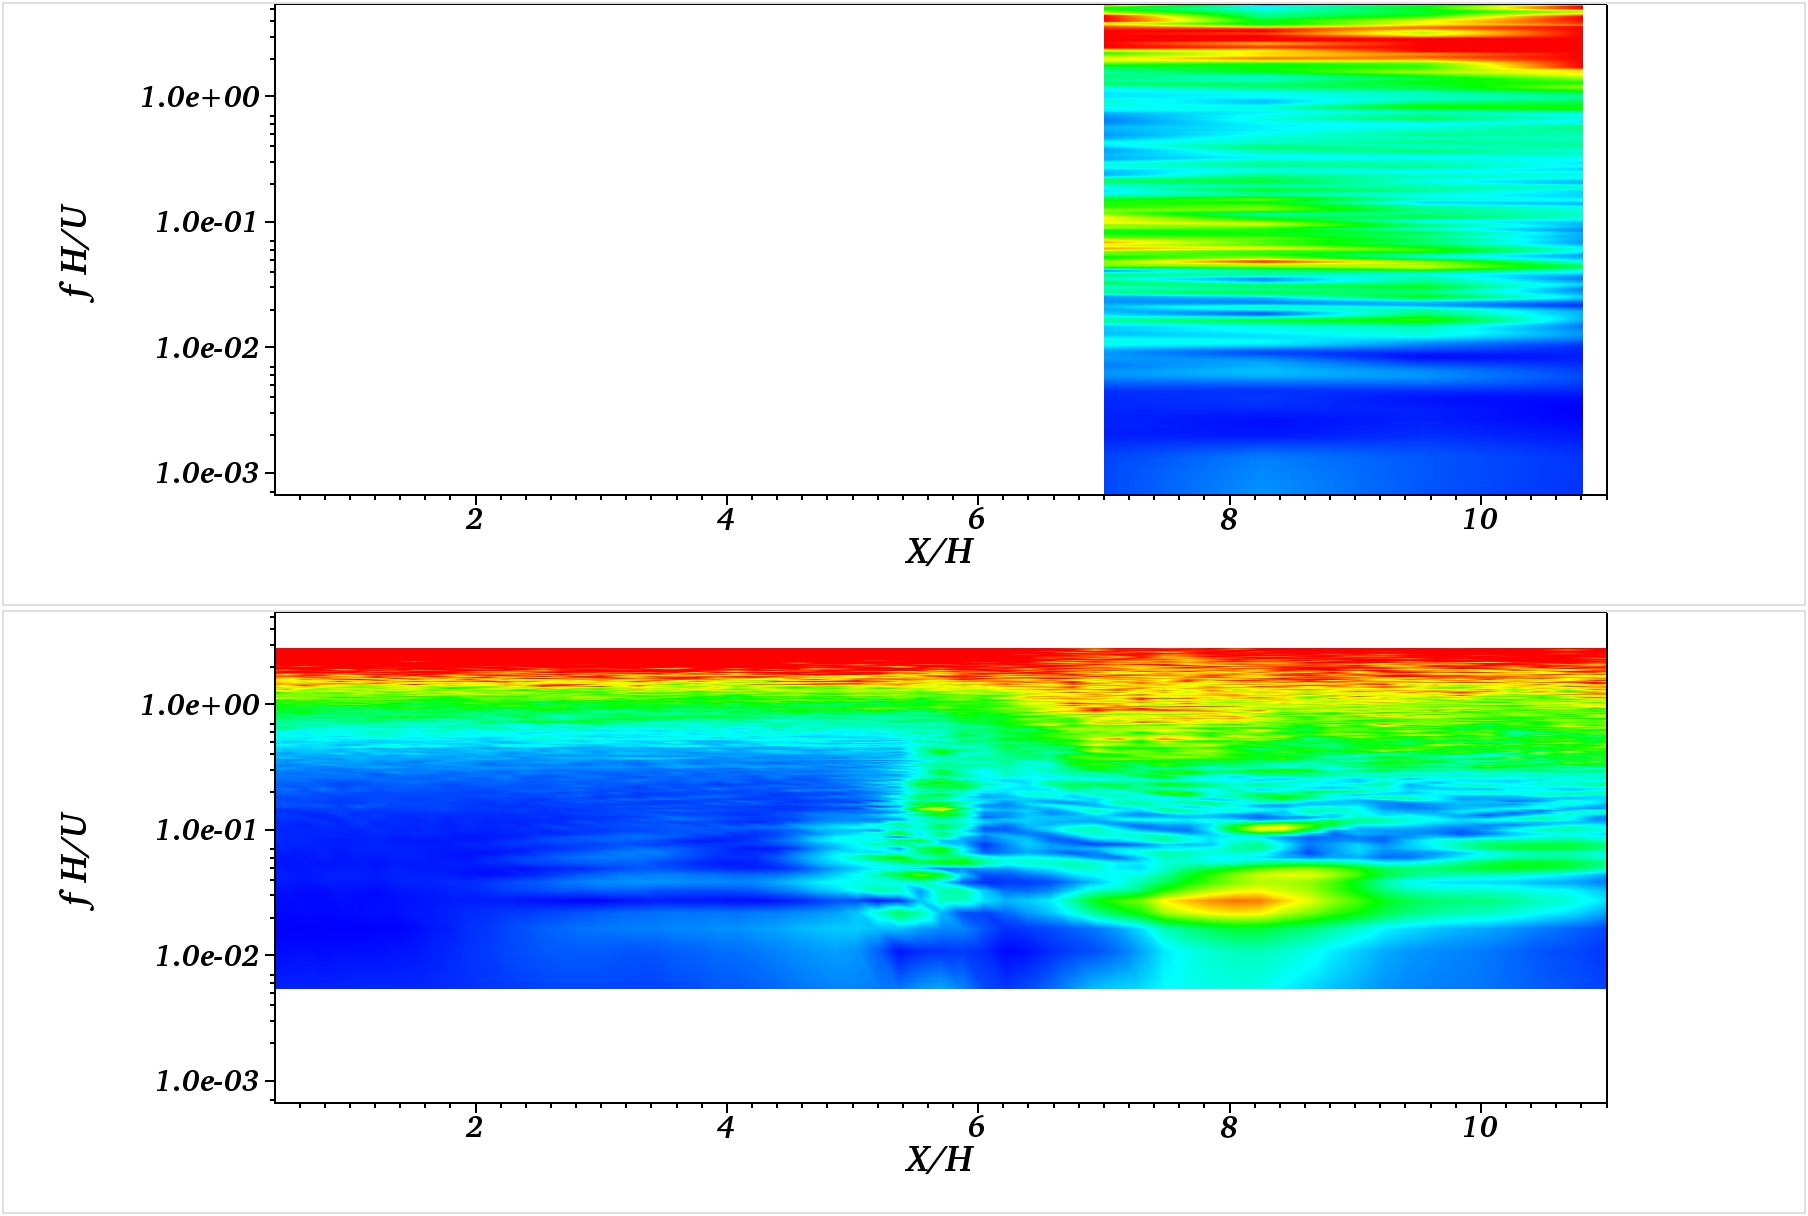
\includegraphics[height=2.5in]{../../figs/XvSt_wall.jpg}}
	\subfloat[(b)] { \label{fig:var_comp} \includegraphics[height=2.in]{../../figs/p_var.pdf} }
	\caption{ {\bf Left:} Compensated energy spectra for wall pressure fluctuations normalized such that the integral over frequency at each $x$ location is unity.  Experimental data (top) and LES case A data (bottom) show both depict the low frequency motion of the shock wave and the high frequency turbulent boundary and shear layer. {\bf Right:} Time-averaged pressure variance as a function of $x$ is shown for LES case A (solid line) and the experiment (circles).
 	%\label{fig:comp_spectra}
	}
	%\end{centering}
\end{figure*}



\subsubsection{Time history of shock wave location }

From the instantaneous wall pressure profile, the shock location is determined.  The experimentalists fit the pressure profiles to a curve that approximated the pressure profile across a shock.  Our approach, however, simply tracks the minimum value of pressure along an $x$-profile which was taken at top, bottom and centerline locations in the diverging section of the nozzle.  Figure~\ref{fig:shock_history} shows the temporal behavior of the shock location based on the pressure profiles (top,bottom,center) and illustrates the asymmetry of the shock.  Autospectra of this time history are also shown for the experiment and LES cases A and B in Fig.~\ref{fig:shock_spectra}.  The LES spectra lack in low frequency resolution and as a result, there are discrepancies from the experiment at lower Strouhal numbers.  The case A calculation has nearly 2 times the samples as case B and has a substantially better spectrum at the lower wave numbers.  Capturing more low frequency periods is expected to improve this measure.  

%\end{multicols}


\begin{figure*}[!h]% order of placement preference: here, top, bottom
	%\begin{center}
	\centering
	\subfloat[(a)]{\label{fig:shock_history} 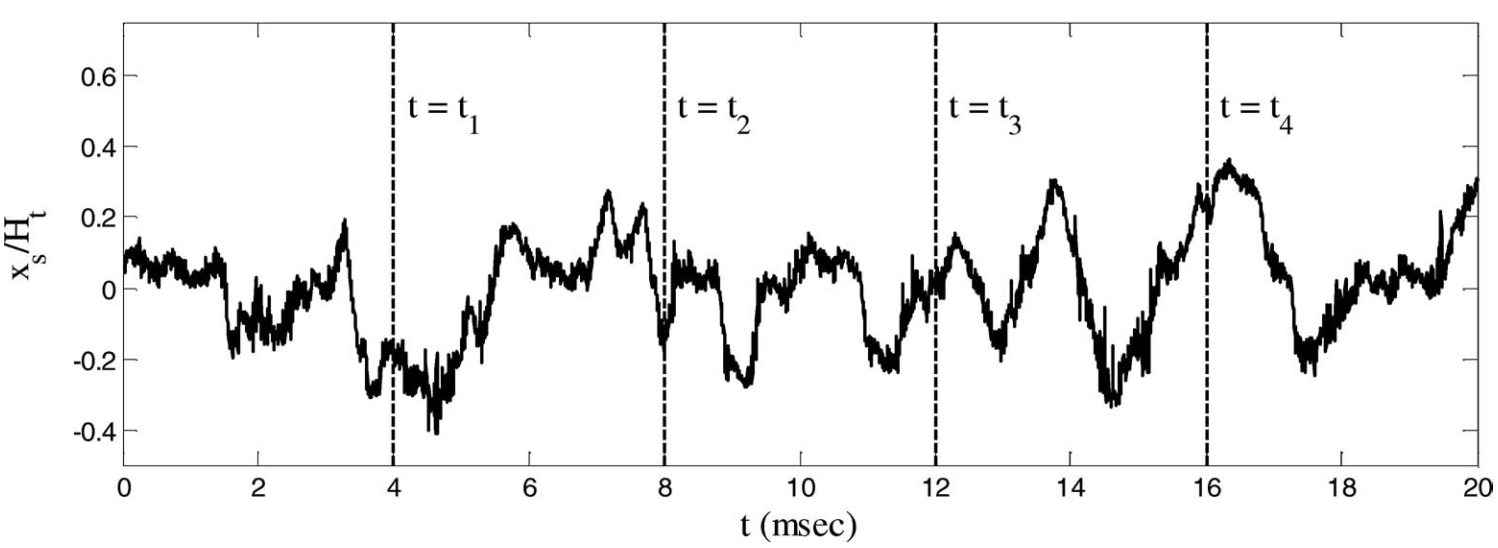
\includegraphics[height=2.5in]{../../figs/shock_history.pdf}}
	\subfloat[(b)]{\label{fig:shock_spectra} \includegraphics[height=2.5in]{../../figs/shock_spectra.pdf}}
	%\end{center}
 	\caption{ {\bf Left}: Shock location vs. time based on pressure profiles at three locations for LES case A. {\bf Right:} Autospectra of shock position fluctuation for the experiment (dashed-black), LES case A (dashed dot-red) and LES case B(dashed-dot blue) mesh calculations. }
 	
\end{figure*}


\begin{figure*}[!h]
	\begin{centering}
	\includegraphics[width=6.5in, height=2.5in, keepaspectratio=false]{../../figs/shock_compare.pdf}
	\caption{ Shock wave position time history from the experimental measurements~\cite{Papam:10} are shown as the original figure in black.  The over-layed red line represents data from case A of the LES and shows good qualitative agreement.
 	\label{fig:shock_compare}
	}
	\end{centering}
\end{figure*}


%\begin{multicols}{2}

\subsubsection{Schlieren}


Figures~\ref{fig:schl} and~\ref{fig:schl_ex} show a comparison between Schlieren photographs taken from the experiment and results taken from the mesh B calculation in the diverging and exit sections of the nozzle.  Contours of instantaneous span averaged density gradient magnitude ($||\nabla\rho|| $) show that the LES calculation is in good qualitative agreement with the experiment.  The shock location, (which was experimentally reported to oscillate left and right by a distance of +/- $\delta_N$ ) agrees quite well with the experiment.  Furthermore the secondary shocks or the ``aftershocks'' observed in the experiment are captured.  The asymmetry of the lambda shock as well as the separated shear layers are clearly represented.


%\end{multicols}
%\clearpage

\begin{figure}[!h]% order of placement preference: here, top, bottom
	\begin{center}
	\subfloat[(a)]{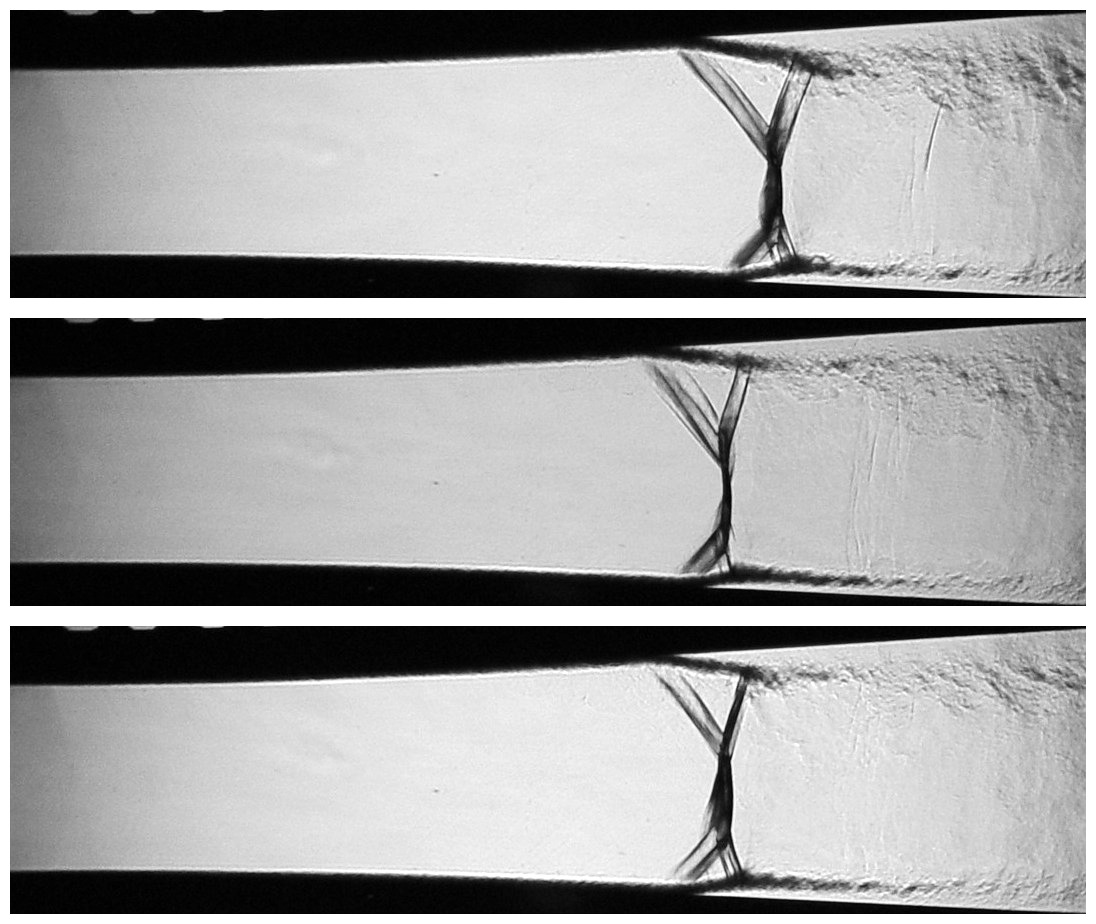
\includegraphics[width=3in]{../../figs/exp_montage.jpg}}
	\subfloat[(b)]{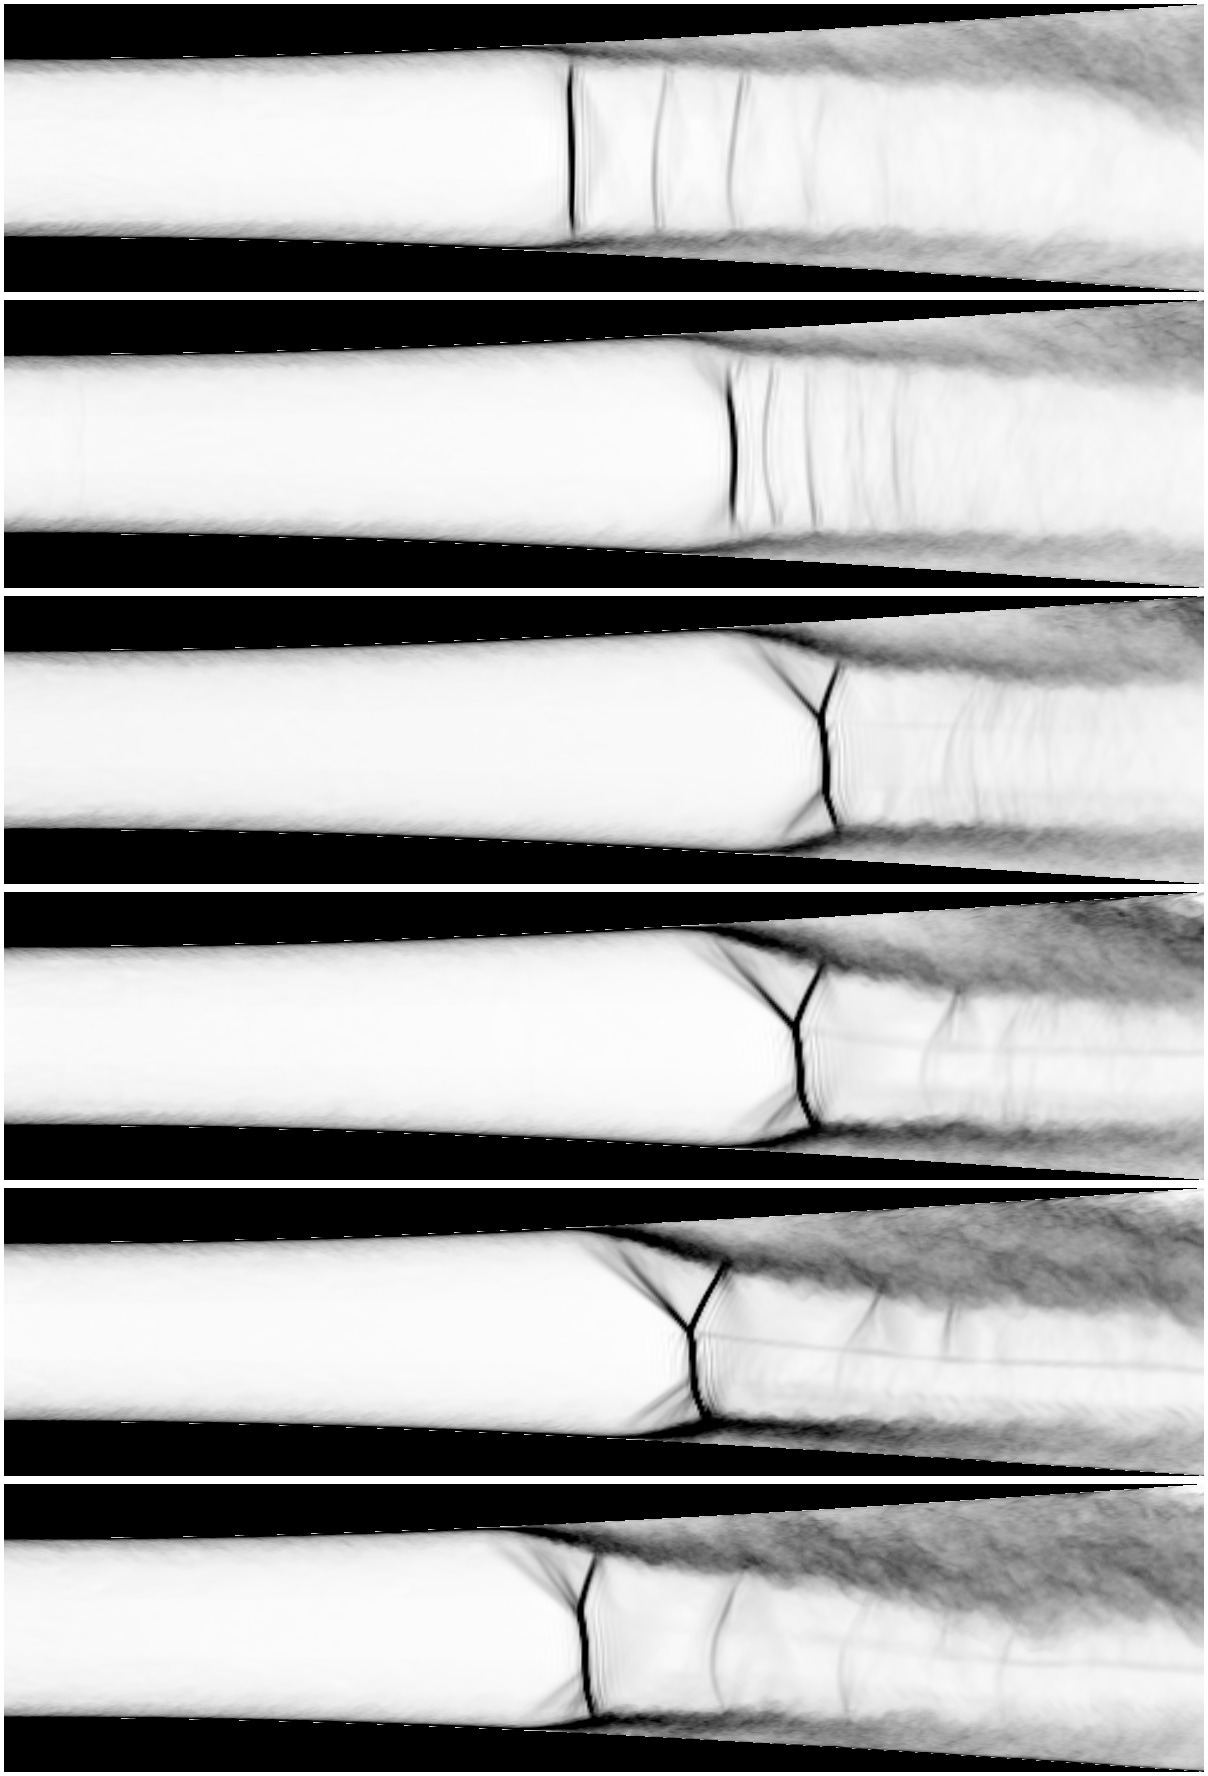
\includegraphics[width=3in]{../../figs/sim_montage.jpg}}
	\end{center}
 	\caption{Schlieren images from experiment \cite{Papam:10} (left) and $z$-averaged contours of $||\nabla\rho||$ from mesh B of the LES (right) show excellent qualitative agreement of the shock structure, the separated shear layer and the compression/expansion waves.  }
 	\label{fig:schl}
\end{figure}


\begin{figure}[!h]% order of placement preference: here, top, bottom
	\begin{center}
	\subfloat[(a)]{\includegraphics[height=3in, angle=-90]{figs/plume_exp.png}}
	\subfloat[(b)]{\includegraphics[height=3in, angle=-90]{figs/plume_les.png}}
	\end{center}
 	\caption{Schlieren images from experiment \cite{Papam:10} (left) and $z$-averaged contours of $||\nabla\rho||$ from mesh B of the LES (right) in the exit region of the diverging section of the nozzle.  }
 	\label{fig:schl_ex}
\end{figure}


%\begin{multicols}{2}
\section{Low Frequency Motion of the Shock}

One of the main findings of the experiment~\cite{Papam:10} was the correlation between the large separated shear layer and the shock wave location.  Intuitively, the total pressure fluctuations in the shear layer became more intense as the shock became stronger and located further downstream.   The effect of the compression/expansion waves downstream of the shock was found to have little effect on the shear layer.

From the LES data, we have observed results consistent with the experimental findings.  Although the experimental data corroborate the LES findings, no cause or mechanism for the shock motion was given.  Indeed with the limited temporal and spatial dimensions and flow-variables measured in the experiment, such conclusions are difficult to make.  Informed by the LES data, we offer here a candidate explanation of the physical mechanism which couples the shock and the shear layer and which governs the shock motion and downstream exit plume mixing.


This mechanism is best understood by visualizing one low frequency period of the shock motion.  Figure~\ref{fig:history} shows the shock structure and separated shear layer in black and white and the region of reversed flow where $U<0$ is shown is color.  The sequence of events leading to one low frequency period goes as follows:  

%Shock is at its most upstream location, and weakest at $\tau=37.1$ ($6^{th}$) snapshot) . From this time moving forward (over a cycle) and coming to snapshot 1 after 4 frames the shock is nearly normal, the boundary layer on the bottom wall mildly separates (incipient separation with no mean reversed flow) and we have a weak separation shock. During this phase the exit pressure decreases and the exit velocity increases (both with different phase delays). From here on going to snapshot 2 a significant reversed flow begins, the separation shock intensifies, the shear layer deflects and the exit area blockage increases. Increased blockage raises exit pressure and even under-expanded state as the reversed flow keeps building strength (snaphots 3 and 4) and then the normal shock begins moving upstream allowing the exit pressure to drop, exit velocity to increase which eliminate the reversed flow.

%As the shock location reaches its furthest downstream position,($\tau=7.4$), the


%The shock wave is located upstream of its mean position and the nozzle is under-expanded (i.e. the exit pressure is higher than the ambient pressure).  At this location, the shock is weaker and it does not create any flow reversal.  The effect of mismatched pressure forces the shock downstream.  

At $\tau=0.0$ the shock is traversing downstream and the incipient separation (with no mean flow reversal) is mild.  As the shock moves further downstream, the Mach number of the shock increases and the larger adverse pressure gradient across the shock causes the flow to begin to reverse ($\tau=7.4$).  The reversed flow causes the shear layer to dramatically thicken.  This thickening obstructs the core mean flow and decreases the effective area of the exit.  As area decreases, the flow accelerates and the pressure drops, as in quasi-1d subsonic flow ($\tau=14.8-29.7$).  To compensate for the area confinement and pressure drop, the shock begins to move upstream as it adjusts to increase pressure with some characteristic time lag ($\tau=14.8-37.1$).  The shock strength is weaker upstream and the separated shear layer becomes milder and the flow ceases to reverse, thus alleviating the confinement from the large shear layer.  As the effective area is increased, the exit pressure becomes larger than the ambient pressure and the shock moves downstream ($\tau=44.5-51.9$).   The cycle then repeats.

The aforementioned mechanism for the low frequency shock motion is summarized below and makes reference to the times and features shown in Figure~\ref{fig:history}.
\begin{itemize}
	%\item Shock is upstream \& $P_e > P_{\infty}$. ($\tau=0$)
	\item Shock moves downstream, mean flow reversal occurs. ($\tau=0-7.4$)
	\item Shear layer thickens, causing blockage \& reduced area. ($\tau=14.8-22.2$)
	\item Area reduction decreases pressure \& $P_e < P_{\infty}$ ($\tau=22.2-29.7$)
	\item Shock moves upstream, flow reattaches. ($\tau=37.1$)
	\item Shear layer thins, relieving blockage \& increase area. ($\tau=44.5$)
	\item Area increase increases pressure \& $P_e > P_{\infty}$ ($\tau=44.5-51.9$)
	\item Shock moves downstream, cycle repeats ($\tau=51.9-56.06$)
\end{itemize}

\begin{figure}[!ht]
  \centering
  
  
  \subfloat[$\tau=0$]{\includegraphics[width=2in]{figs/medium_figs/medium3dgradRHO_sep_0550.png}}    
  \hspace{0.1in}	            
  \subfloat[$\tau=22.2$]{\includegraphics[width=2in]{figs/medium_figs/medium3dgradRHO_sep_0700.png}}
  \hspace{0.1in}	
  \subfloat[$\tau=44.5$]{\includegraphics[width=2in]{figs/medium_figs/medium3dgradRHO_sep_0850.png}}
  
  \vspace{-.1in}
  
  \subfloat[$\tau=7.4$]{\includegraphics[width=2in]{figs/medium_figs/medium3dgradRHO_sep_0600.png}}    
  \hspace{0.1in}	            
  \subfloat[$\tau=29.7$]{\includegraphics[width=2in]{figs/medium_figs/medium3dgradRHO_sep_0750.png}}
  \hspace{0.1in}	
  \subfloat[$\tau=51.9$]{\includegraphics[width=2in]{figs/medium_figs/medium3dgradRHO_sep_0900.png}}
  
  \vspace{-.1in}
  
  \subfloat[$\tau=14.8$]{\includegraphics[width=2in]{figs/medium_figs/medium3dgradRHO_sep_0650.png}}    
  \hspace{0.1in}	            
  \subfloat[$\tau=37.1$]{\includegraphics[width=2in]{figs/medium_figs/medium3dgradRHO_sep_0800.png}}
  \hspace{0.1in}	
  \subfloat[$\tau=56.06$]{\includegraphics[width=2in]{figs/medium_figs/medium3dgradRHO_sep_0928.png}}
  
  \caption{Shock wave motion and the corresponding separated shear layer over one low-frequency period.  Contours of $||\nabla\rho||$ are shown in grayscale and colored regions depict negative $U$ velocity, where red represents a Mach number of approximately 0.1 and blue is zero.   }
  
  \label{fig:history}
\end{figure}



\begin{figure}[!h]% order of placement preference: here, top, bottom
	\begin{center}
	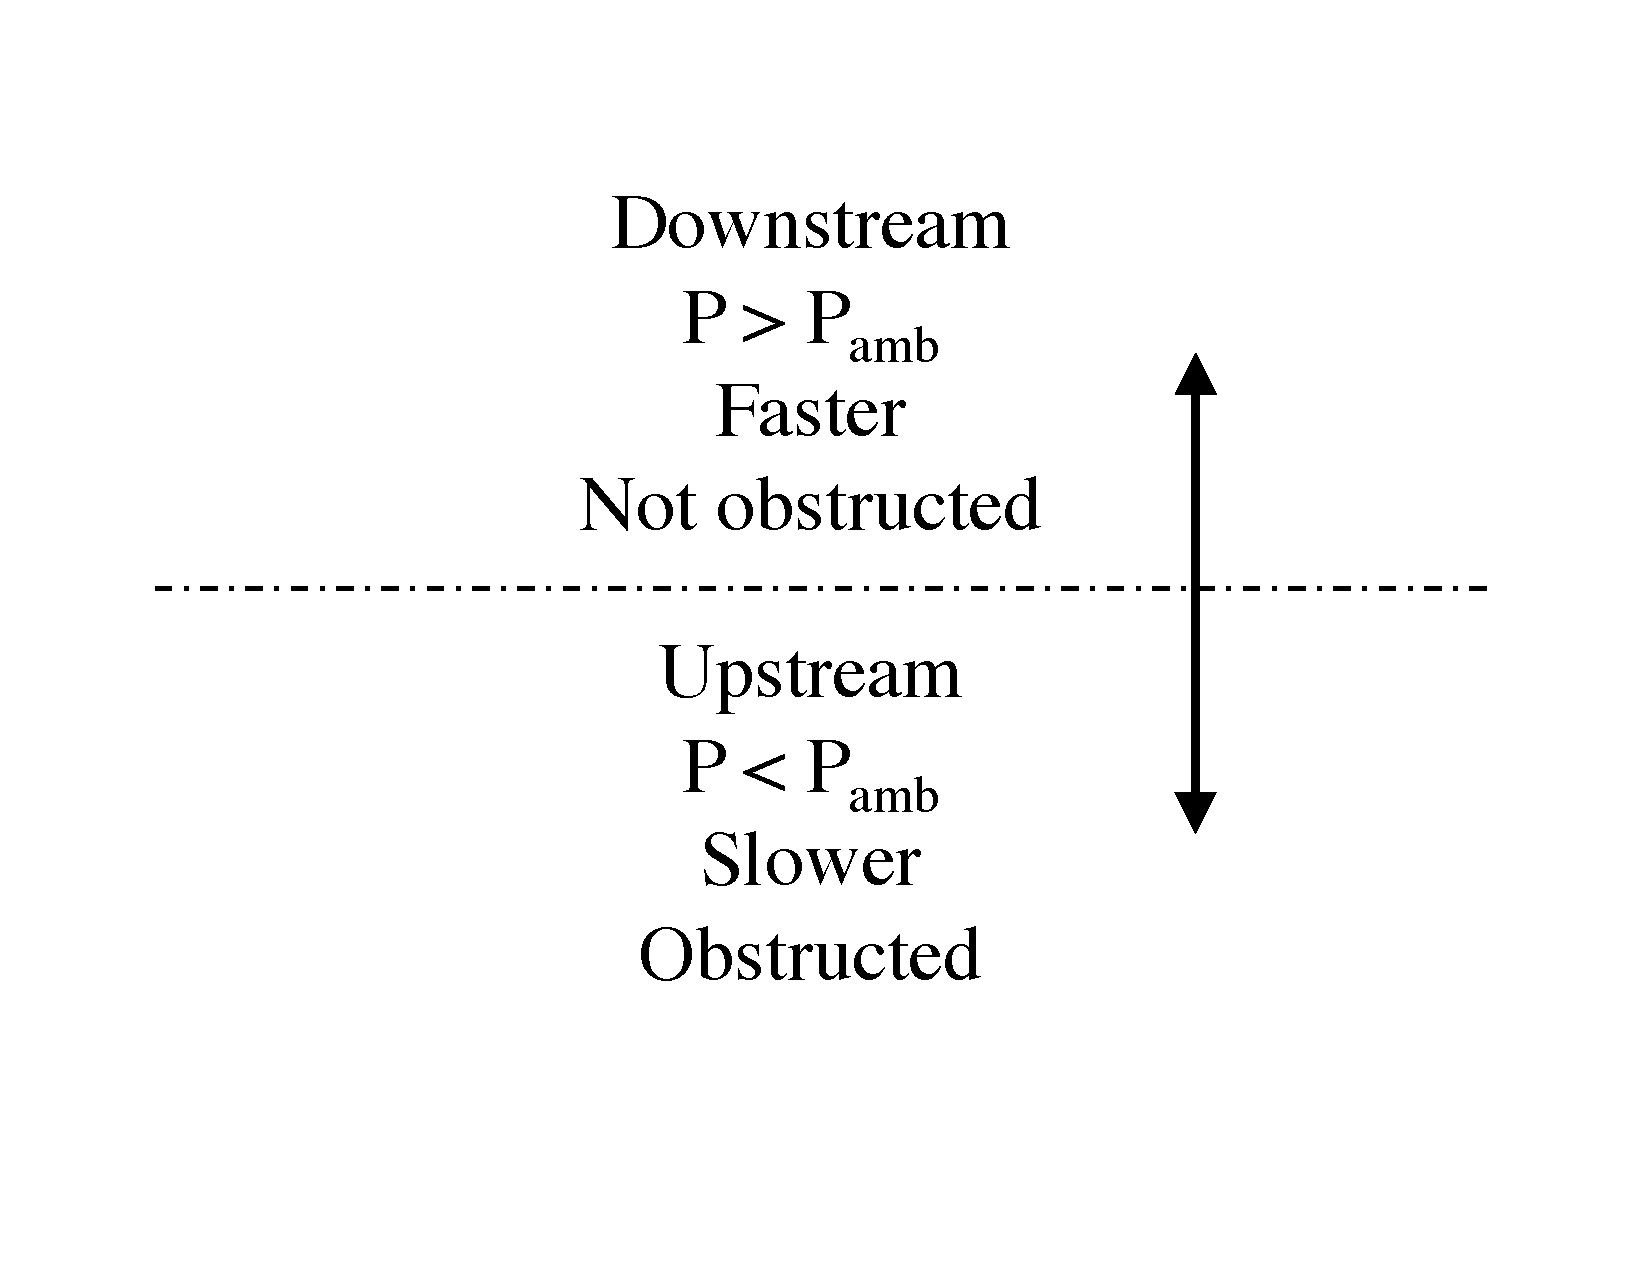
\includegraphics[trim = 3in 0in 2in 0in, clip,width=2.085in]{figs/phase_key.pdf}
	\includegraphics[width=3.5in]{../../figs/mech_phase.pdf}
	\end{center}
 	\caption{Time histories of shock position, exit pressure, exit velocity and effective exit area.  The key to the left of the plot indicates for each variable or quantity what a positive or negative value on the plot represents.  Data has been low-pass filtered to bring focus on the low-frequency motion and normalized to show trends and time relationships.  Phase lag between shock position (black) and effective exit area (green) is clearly shown.  Pressure and velocity (shown in blue and red respectively) have other modes present in their behavior.  Red dots correspond to the images of Fig.~\ref{fig:history} and \ref{fig:whistory}   }
 	\label{fig:phase}
\end{figure}


\begin{figure}[!ht]
  \centering
  
  
  \subfloat[$\tau=0$]{\includegraphics[width=2in]{figs/med_Mach/medium3dMach_0550.png}}    
  \hspace{0.1in}	            
  \subfloat[$\tau=22.2$]{\includegraphics[width=2in]{figs/med_Mach/medium3dMach_0700.png}}
  \hspace{0.1in}	
  \subfloat[$\tau=44.5$]{\includegraphics[width=2in]{figs/med_Mach/medium3dMach_0850.png}}
  
  \vspace{-.1in}
  
  \subfloat[$\tau=7.4$]{\includegraphics[width=2in]{figs/med_Mach/medium3dMach_0600.png}}    
  \hspace{0.1in}	            
  \subfloat[$\tau=29.7$]{\includegraphics[width=2in]{figs/med_Mach/medium3dMach_0750.png}}
  \hspace{0.1in}	
  \subfloat[$\tau=51.9$]{\includegraphics[width=2in]{figs/med_Mach/medium3dMach_0900.png}}
  
  \vspace{-.1in}
  
  \subfloat[$\tau=14.8$]{\includegraphics[width=2in]{figs/med_Mach/medium3dMach_0650.png}}    
  \hspace{0.1in}	            
  \subfloat[$\tau=37.1$]{\includegraphics[width=2in]{figs/med_Mach/medium3dMach_0800.png}}
  \hspace{0.1in}	
  \subfloat[$\tau=56.06$]{\includegraphics[width=2in]{figs/med_Mach/medium3dMach_0928.png}}
  
  \caption{Contours of Mach number from 0 (blue) to 1.5 (red) and sonic line (black line) show the supersonic and subsonic regions of flow in the nozzle.  Small localized regions of the flow downstream of the shock are supersonic.  The Mach number at the exit is always subsonic.}
  
  \label{fig:mhistory}
\end{figure}


\begin{figure*}
  \centering
  
  \subfloat[$\tau=0$]{\includegraphics[width=2in]{figs/wall/medium3dwall_0550.png}}    
  \hspace{0.1in}	            
  \subfloat[$\tau=22.2$]{\includegraphics[width=2in]{figs/wall/medium3dwall_0700.png}}
  \hspace{0.1in}	
  \subfloat[$\tau=44.5$]{\includegraphics[width=2in]{figs/wall/medium3dwall_0850.png}}
  
  
  \subfloat[$\tau=7.4$]{\includegraphics[width=2in]{figs/wall/medium3dwall_0600.png}}    
  \hspace{0.1in}	            
  \subfloat[$\tau=29.7$]{\includegraphics[width=2in]{figs/wall/medium3dwall_0750.png}}
  \hspace{0.1in}	
  \subfloat[$\tau=51.9$]{\includegraphics[width=2in]{figs/wall/medium3dwall_0900.png}}
  
  
  \subfloat[$\tau=14.8$]{\includegraphics[width=2in]{figs/wall/medium3dwall_0650.png}}    
  \hspace{0.1in}	            
  \subfloat[$\tau=37.1$]{\includegraphics[width=2in]{figs/wall/medium3dwall_0800.png}}
  \hspace{0.1in}	
  \subfloat[$\tau=56.06$]{\includegraphics[width=2in]{figs/wall/medium3dwall_0928.png}}
  
  \caption{Grayscale is $C_f$ from -0.01 to 0.01 corresponding from black to white.  Colored region are contours of temperature on a range from $.56T_{\infty}$ to $.94T_{\infty}$ which have been thresholded to not show values below $.60T_{\infty}$.  The entrainment of the hot air by the separated flow is clearly illustrated as the shock undulates.  }
  
  \label{fig:whistory}
\end{figure*}

%\begin{multicols}{2}
The separated shear layer is coupled to the shock wave position, expanding to force the shock upstream and contracting to allow the shock to traverse downstream.  During this motion there is an observed latency between shock re-location and shear layer reattachment or separation.  The phase shift of the two motions cause the cycle to constantly over compensate in its adjustments to match exit pressure and hence the motion is inherently unstable.  This phase lag can be seen in Figure~\ref{fig:phase} where low-pass filtered time histories of the shock position, effective area at the exit (due to constriction of the shear layers), exit pressure and exit velocity are shown.  All quantities have been normalized such that they oscillate about zero, and don't exceed unity on either extreme.  Units are inconsequential for illustrating the fluctuating trends and behavior of the quantities.

This cycle occurs on a broad range of time and length scales.  The advancing or retreating of the shock is dictated by the separating or reattaching of the shear layer.  It has been shown (Fig.~\ref{fig:PSD_comp}) that the total pressure spectrum in the shear layer is broad-band and correlates strongly with the shock motion.

The breathing of the shear layer is further illustrated in Figure~\ref{fig:whistory} which shows the friction coefficient, $C_f$ in black and white and contours of temperature above $0.6 \ T_{\infty}$ on a two dimensional projection of the nozzle wall.  Temperature above this value is only found in the ambient flow field, hence its presence in the nozzle is a good surrogate tracer for reversed flow.  Hot gas is sucked in as the flow separates and then pushed out as the flow reattaches.




\section{Conclusion}
We have conducted a series of LES calculations to model an experiment~\cite{Papam:10} of a shock boundary layer interaction in a planar nozzle.  The LES data show excellent agreement with the reported experimental results and indicate that the proper physics are being captured by the LES model.  Convergence studies show that the turbulent boundary layer is sufficiently resolved near the wall.  The unsteady motion of the shock is accurately represented by the LES, although the lower frequencies have yet to be sufficiently resolved.  We proposed an intuitive mechanism for the unsteady shock motion which couples the shock location, shear layer instability and separated region and which agrees with the conclusions made by Johnson and Papamoschou.  Although the  mechanism has only thus far been supported by observation, the richness of the LES data will allow for a much more in depth analysis of the unsteady flow physics and allow for further advances in the understanding of shock-boundary layer interactions. 



\section*{Acknowledgments}

This work is supported by the Department of Energy SciDAC2 Grant (Grant DE-FC02-06-ER25787) and the DOE Computational Science Graduate Fellowship (CSGF) with computational resources provided by Lawrence Livermore National Lab.  Thanks is given to Dr. A. Cook and Dr. W. Cabot for providing the code which was modified for the present study.  The authors also express their gratitude to Dr. Andrew Johnson and Prof. Dimitri Papamoschou for their generous sharing of experimental data and many valuable discussions.

\begin{thebibliography}{10}% maximum number of references (for label width)
 
 \bibitem{Lele:92}
 	S.K. Lele, ``Compact Finite-Difference Schemes With Spectral-Like Resolution,'' \emph{Journal of Computational
	Physics}, Vol. 103, pp. 16-42, 1992.
	
\bibitem{Poinsot:92}
	T.J. Poinsot and S.K. Lele, ``Boundary conditions for direct simulations of compressible viscous flow,'' \emph{Journal of Computational Physics}, 101(1):104-129, 1992

 \bibitem{Cook:07} 
 	A.W. Cook,  ``Artificial Fluid Properties for large-eddy simulation of compressible turbulent mixing,'' \emph{Physics of Fluids}, Volume {\bf 19}, 2007.
	
\bibitem{CookCabot:05}
	A.W. Cook and W.H. Cabot, ``Hyperviscosity for shock-turbulence interactions'', \emph{Journal of Computational Physics}, Vol. 203(2):379-385, 2005
 
 \bibitem{Kawai:10}
 	S. Kawai, S. K. Shankar and S. K. Lele, ``Assessment of localized artificial diffusivity scheme for large-eddy simulation of compressible turbulent flows,'' \emph{Journal of Computational Physics}, {\bf 		229} (5), 1739-1762, (2010).
	
 \bibitem{Kawai:10aiaa}
	S. Kawai, S.K. Lele, ``Large-Eddy Simulation of Jet Mixing in Supersonic Crossflows,'' \emph{AIAA JOURNAL} Vol. 48, No. 9, September 2010.
	
 \bibitem{Touber:09}
 	E. Touber and N.D. Sandham, ``Large-eddy simulation of low-frequency unsteadiness in a turbulent shock-induced separation bubble,'' \emph{Theoretical and Computational Fluid Dynamics} Volume 23, Number 2, 79-107

 \bibitem{Pirozzoli:09}
 	S. Pirozzoli, A. Beer, M. Bernardini and F. Grasso, ``Computational analysis of impinging shock-wave boundary layer interaction under conditions of incipient separation,'' \emph{Shock Waves} Volume 19, Number 6, 487-497

 \bibitem{Kennedy:00}
 	C.A. Kennedy, M.H. Carpenter and R.M. Lewis, ``Low-storage, explicit Runge-Kutta schemes for the compressible Navier-Stokes equations,'' \emph{Appl. Numer. Math.} {\bf 35}, 177 (2000) 
 
 \bibitem{Ostlund:05}
 	J. Ostlund and B. Muhammad-Klingmann,``Supersonic flow separation with application to rocket engine nozzles,'' \emph{Appl. Mech. Rev.} {\bf 58}, 143 (2005).
 
 \bibitem{Papam:10}
 	A.D. Johnson and D. Papamoschou, ``Instability of shock-induced nozzle flow separation,'' \emph{Physics of Fluids}, Volume {\bf 22}, (2010).
	
 \bibitem{Papam:09}
 	D. Papamoschou, A. Zill, A. Johnson, ``Supersonic flow separation in planar nozzles,'' \emph{Shock Waves}, {\bf 19}, 171 (2009).

 \bibitem{Xiao:07}
 	Q. Xiao, H.M. Tsai and D. Papamoschou, ``Numerical investigation of supersonic flow separation,'' \emph{AIAA J.} {\bf 45}, 532 (2007).
	
 \bibitem{Papam:06}
 	D. Papamoschou and A. Johnson, ``Unsteady phenomena in supersonic nozzle flow separation,'' \emph{AIAA J.} 2006-3360, (2006).
	
 \bibitem{Bourgoing:05}
 	A. Bourgoing and Ph. Reijasse, ``Experimental analysis of unsteady separated flows in a super-sonic planar nozzle,'' \emph{Shock Waves} {\bf 14}, 251 (2005).
	
 \bibitem{Dussauge:09}
 	S. Piponniau, J.P. Dussauge, J.F. Debieve and P. Dupont, ``A simple model for low-frequency unsteadiness in shock induced separation,'' \emph{J. Fluid Mech.}, vol. {\bf 629}, pp. 87-108 (2009).
	
 \bibitem{Lund:98}
 	T.S. Lund, X. Wu, and K.D. Squires, ``Generation of Turbulent Inflow Data for Spatially-Developing Boundary Layer 
Simulations,'' \emph{Journal of Computational Physics}, Vol. 140, No. 2, 1998, pp. 233-258.

\bibitem{Urban:01}
	G. Urban, D. Knight, ``Large-Eddy Simulation of a Supersonic Boundary Layer Using an Unstructured Grid'', \emph{AIAA JOURNAL} {\bf Vol.} 39, No. 7, July 2001

 %\bibitem{Morgan:10a} 
% 	B. Morgan, J. Larsson, S. Kawai and S.K. Lele, ``An Improved Method for Prescribing Turbulent Boundary Layer 
%Inflow'', \emph{AIAA Journal}, submitted for publication, June, 2010.

 \bibitem{Morgan:10b} 
 	B. Morgan,S. Kawai and S.K. Lele, ``Large-Eddy Simulation of an Oblique Shock Impinging on a 
Turbulent Boundary Layer'', \emph{AIAA Journal}, 2010-4467, 2010.
 	
 \bibitem{Bookey:05}
 	P.B. Bookey, C. Wyckham, A.J. Smits, and M.P. Martin, ``New Experimental Data of STBLI at DNS/LES Accessible 
Reynolds Numbers,''  AIAA Paper 2005-309, Jan. 2005.

\bibitem{Spalart:93}
	P. Spalart and J. Watmuff, ``Experimental and numerical study of a turbulent boundary layer with pressure gradients,'' \emph{J. Fluid Mech.},
vol. {\bf 249}, pp. 337-371 (1993)	

\bibitem{Dixit:08}
	S.A. Dixit, O.N. Ramesh, ``Pressure-gradient-dependent logarithmic laws in sink flow turbulent boundary layers,'' \emph{J. Fluid Mech.}, vol {\bf 615}, pp. 445-475 (2008)

 
	
\end{thebibliography}


\end{document}

% - Release $Name:  $ -
